\documentclass[12pt]{beamer}
\usetheme{Boadilla}
\usepackage{booktabs}
\usepackage{enumitem}
\usepackage{tikz}
\newcommand{\E}{\mathbb{E}}
\usefonttheme{professionalfonts}
\usepackage{pgfplots}
\renewcommand{\arraystretch}{1.25}
\usetikzlibrary{trees}
\title[ECON2843]{Lecture 8}
\subtitle{Part 2 Probability and Distributions}
\date{}
\usepackage{amsmath,amssymb,mathtools,wasysym}
\begin{document}
	\begin{frame}
		\titlepage
	\end{frame}

\begin{frame}
	\frametitle{Example}
	
	\begin{itemize}
		\item[\color{blue}$\blacktriangleright$] A student sitting a statistics quiz decides to answer each of the ten multiple choice questions entirely by chance.
		
		\item[\color{blue}$\blacktriangleright$]Each question has five options, only one of which is correct.
		
		\item[\color{blue}$\blacktriangleright$]Let $X$ be the number of questions the student answers correctly.
		
		\item[\color{blue}$\blacktriangleright$]Then $X \sim Bin(n = 10, p = 0.2)$.
	\end{itemize}
	
\end{frame}
\begin{frame}
	\frametitle{Example}
	
	\begin{itemize}
		\item What is the probability the student gets half the answers correct?
		\[ P(X = 5) = \frac{10!}{5!(10-5)!} \times 0.2^5 \times (1-0.2)^5 = 0.0264 \]
		
		\item What is the probability that the student passes, i.e., gets five or more correct?
		\[ P(X \geq 5) = P(X = 5) + P(X = 6) + P(X = 7) \]
		\[ + P(X = 8) + P(X = 9) + P(X = 10) \]
		\[ = \text{a lot of calculations!} \]
	\end{itemize}
	
\end{frame}

\begin{frame}
	\frametitle{Binomial Tables}
	
	\begin{itemize}
		\item[\color{blue}$\blacktriangleright$] There are tables available that list $P(X \leq k)$ for different values of $k$, $n$ and $p$.
		\item[\color{blue}$\blacktriangleright$] From tables, look up $n = 10$ and $p = 0.2$.
	\end{itemize}
	
	\vspace{0.5cm}
	
	\begin{align*}
		P(X \geq 5) &= 1 - P(X \leq 4) \\
		&= 1 - 0.9672 \text{ (from tables)} \\
		&= 0.0328
	\end{align*}
	
\end{frame}

\begin{frame}
	\frametitle{Binomial Tables}
	
	\begin{itemize}
		\item[\color{blue}$\blacktriangleright$] What is the probability the student gets half the answers correct?
	\end{itemize}
	
	\vspace{0.5cm}
	
	\begin{align*}
		P(X = 5) &= P(X \leq 5) - P(X \leq 4) \\
		&= 0.9936 - 0.9672 \text{ (from tables)} \\
		&= 0.0264
	\end{align*}
	
\end{frame}
 \begin{frame}
 	\frametitle{Binomial Tables}
 	
 	\begin{itemize}
 		\item[\color{blue}$\blacktriangleright$] The binomial tables are a tool to make life easier by helping us calculate binomial probabilities for frequently used values of $n$ and $p$.
 		
 		\item[\color{blue}$\blacktriangleright$] However, they are not a substitute for knowing and being able to use the binomial probability distribution formula - not all values of $n$ or $p$ will be tabulated!
 	\end{itemize}
 	
 \end{frame}
 
 
  \begin{frame}
 	
That's all for discrete probability distribution, let's talk about continuous ones now.
 	
 \end{frame}
 \begin{frame}
 	\frametitle{Continuous Random Variable}
 	
 	\begin{itemize}
 		\item[\color{blue}$\blacktriangleright$] A continuous random variable takes on an uncountable number of possible values.
 		\item[\color{blue}$\blacktriangleright$] Cannot list all possible values in any systematic way.
 		\item[\color{blue}$\blacktriangleright$] It is impossible to assign a non-zero probability to each possible value \emph{and} still have all probabilities add up to 1.
 		\item[\color{blue}$\blacktriangleright$] Therefore, for a continuous random variable $X$, the following is true for \emph{any} value of $x$:
 	\end{itemize}
 	
 	\vspace{0.5cm}
 	
 	\[
 	P(X = x) = 0
 	\]
 	
 \end{frame}
 \begin{frame}
 	\frametitle{Continuous Probability Distribution?}
 	
 	\begin{itemize}
 		\item[\color{blue}$\blacktriangleright$] So what do we do about the probability distribution for a continuous random variable?
 		\item[\color{blue}$\blacktriangleright$] Although $P(X = x) = 0$ for any value $x$, it turns out we can find probabilities of the form:
 		\[ P(a < X < b) \]
 		\item Note:
 		\begin{itemize}
 			\item[\color{blue}$\blacktriangleright$] Discrete:
 			\[ P(X \leq x) \neq P(X < x) \]
 			\item[\color{blue}$\blacktriangleright$] Continuous:
 			\[ P(X \leq x) = P(X < x) \]
 		\end{itemize}
 	\end{itemize}
 	
 \end{frame}
 
 \begin{frame}
 	\frametitle{Flashback to Histograms}
 	
 	\begin{itemize}
 		\item[\color{blue}$\blacktriangleright$] Histograms were a useful way to visually display the \emph{distribution} of continuous data.
 		\item[\color{blue}$\blacktriangleright$] Constructing a histogram involved:
 		\begin{itemize}
 			\item[\color{blue}$\blacktriangleright$]Dividing range of possible values into intervals or ``classes''.
 			\item[\color{blue}$\blacktriangleright$] Counting number of observations that fall into each interval.
 			\item[\color{blue}$\blacktriangleright$] Setting height of each interval to be the frequency (count).
 		\end{itemize}
 	\end{itemize}
 	
 \end{frame}
 
 \begin{frame}
 	\frametitle{Flashback to Histograms}
 	
 	\begin{itemize}
 		\item[\color{blue}$\blacktriangleright$] Let's change the height of each interval in the histogram.
 		\item[\color{blue}$\blacktriangleright$] Suppose we instead set the height of each interval to be:
 	\end{itemize}
 	
 	\vspace{0.5cm}
 	
 	\begin{align*}
 		\text{Interval Height} &= \frac{\text{Count}}{\text{Total Count} \times \text{Interval Width}} \\[1em]
 		&= \text{Proportion} \times \frac{1}{\text{Interval Width}}
 	\end{align*}
 	
 \end{frame}
 
\begin{frame}
	\frametitle{Flashback to Histograms}
	
	\begin{itemize}
		\item[\color{blue}$\blacktriangleright$] The area of a rectangle corresponding to any particular interval is equal to:
	\end{itemize}
	
	\vspace{0.5cm}
	
	\begin{align*}
		\text{Area} &= \text{Interval Height} \times \text{Interval Width} \\[0.5em]
		&= \text{Proportion} \times \frac{1}{\text{Interval Width}} \times \text{Interval Width} \\[0.5em]
		&= \text{Proportion}
	\end{align*}
	
	\vspace{0.5cm}
	
	\begin{itemize}
		\item[\color{blue}$\blacktriangleright$] That is, the area of each rectangle is equal to the probability of an observation falling into that interval.
	\end{itemize}
	
\end{frame}
\begin{frame}
	\frametitle{Measure 10,000 Heights}
		\begin{itemize}
		\item[\color{blue}$\blacktriangleright$] Histogram with 10 intervals.
	\end{itemize}
	\centering
	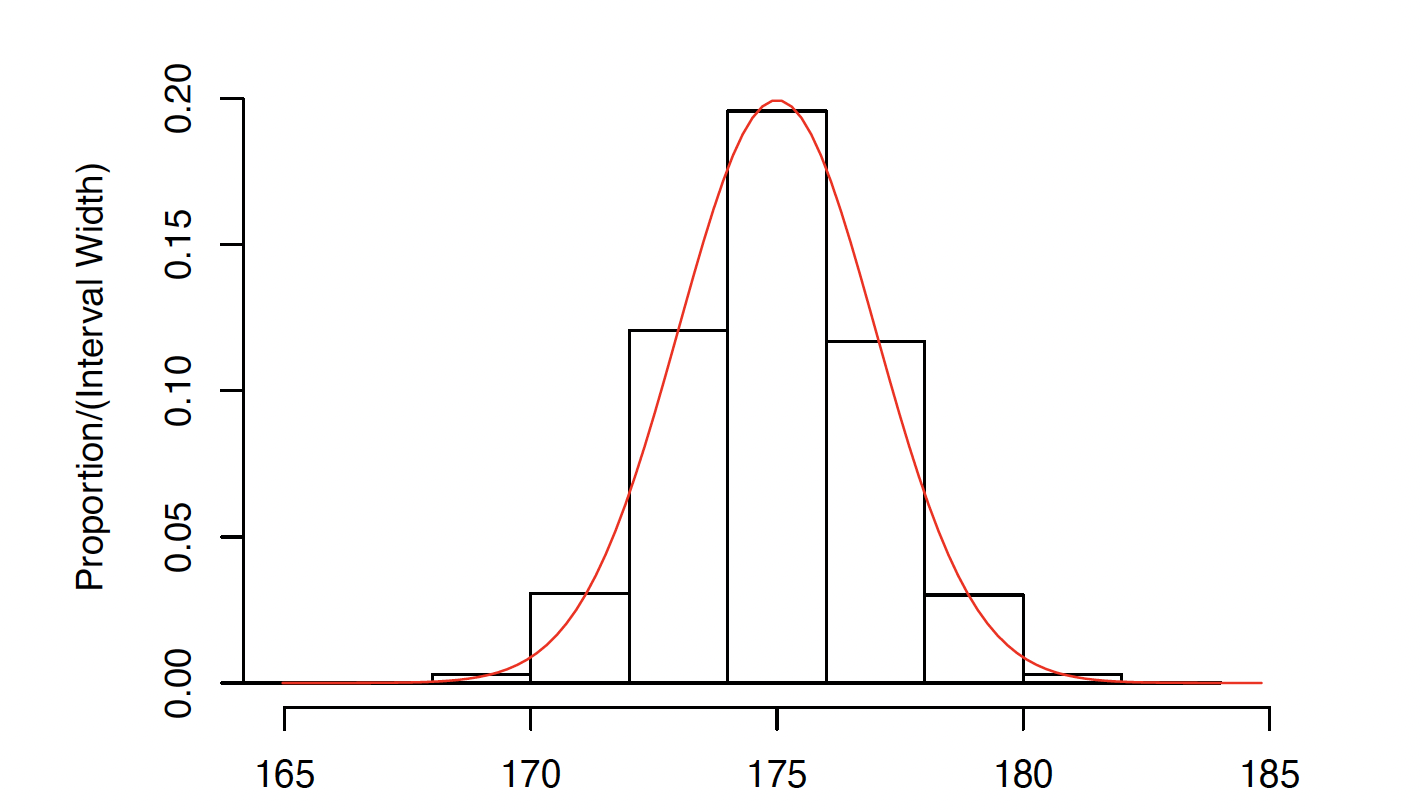
\includegraphics[width=10cm]{histo.png}
\end{frame}
\begin{frame}
	\frametitle{Measure 10,000 Heights}
	\begin{itemize}
		\item[\color{blue}$\blacktriangleright$] Histogram with 50 intervals.
	\end{itemize}
	\centering
	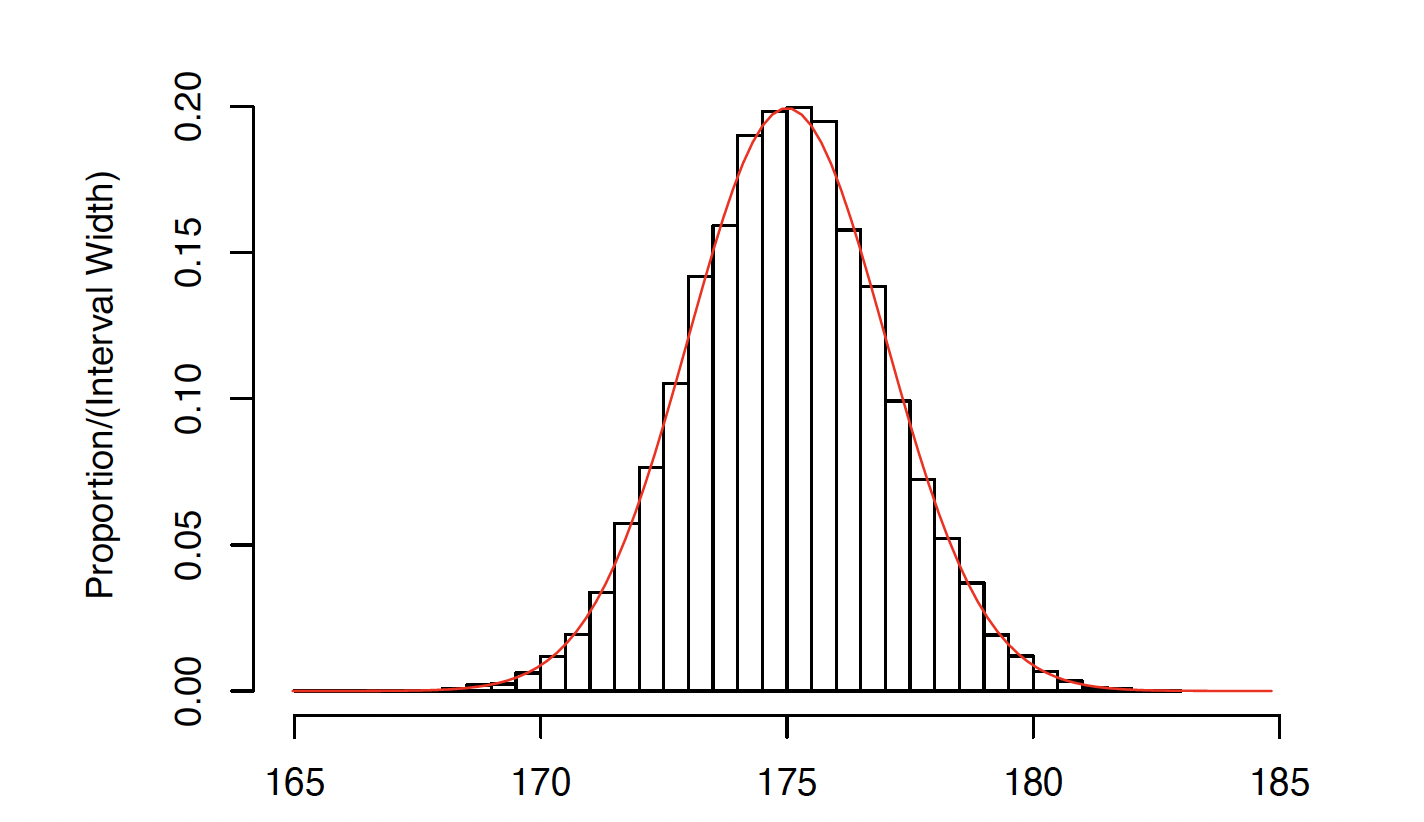
\includegraphics[width=10cm]{histo2.png}
\end{frame}
\begin{frame}
	\frametitle{Measure 10,000 Heights}
	\begin{itemize}
		\item[\color{blue}$\blacktriangleright$] Histogram with 100 intervals.
	\end{itemize}
	\centering
	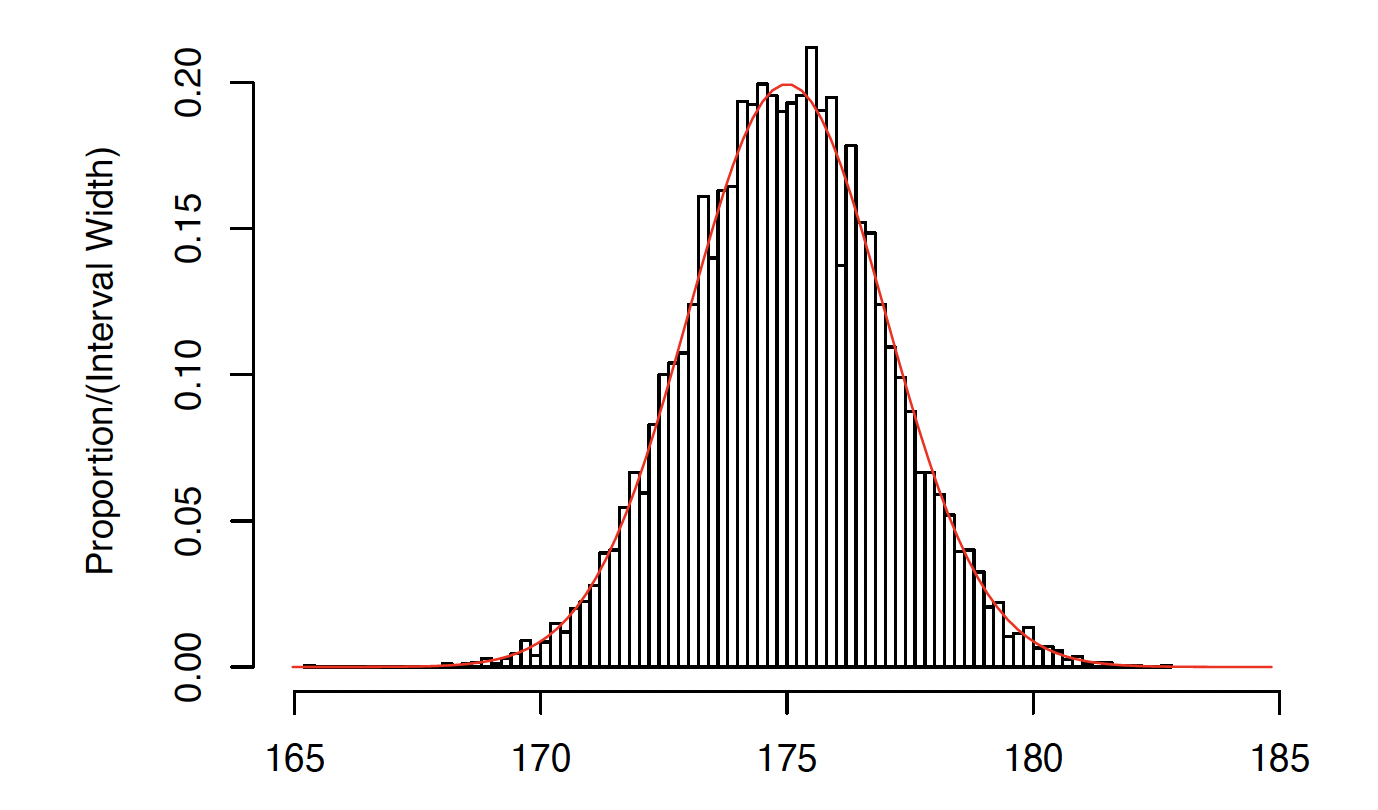
\includegraphics[width=10cm]{histo3.png}
\end{frame}
\begin{frame}
	\frametitle{Measure 100,000 Heights}
	\begin{itemize}
		\item[\color{blue}$\blacktriangleright$] Histogram with 100 intervals.
	\end{itemize}
	\centering
	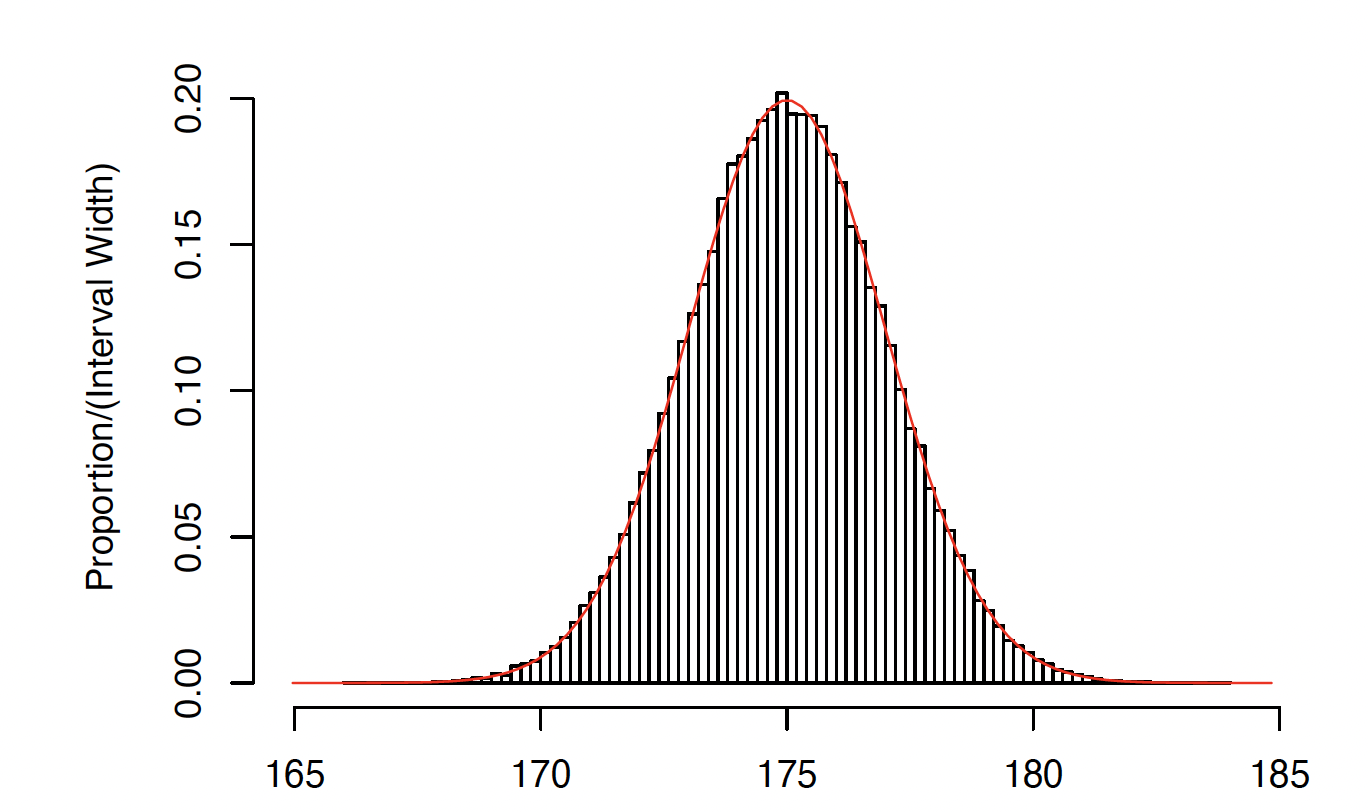
\includegraphics[width=10cm]{histo4.png}
\end{frame}
\begin{frame}
	\frametitle{Measure 1,000,000 Heights}
		\begin{itemize}
		\item[\color{blue}$\blacktriangleright$] Histogram with 100 intervals.
	\end{itemize}
	\centering
	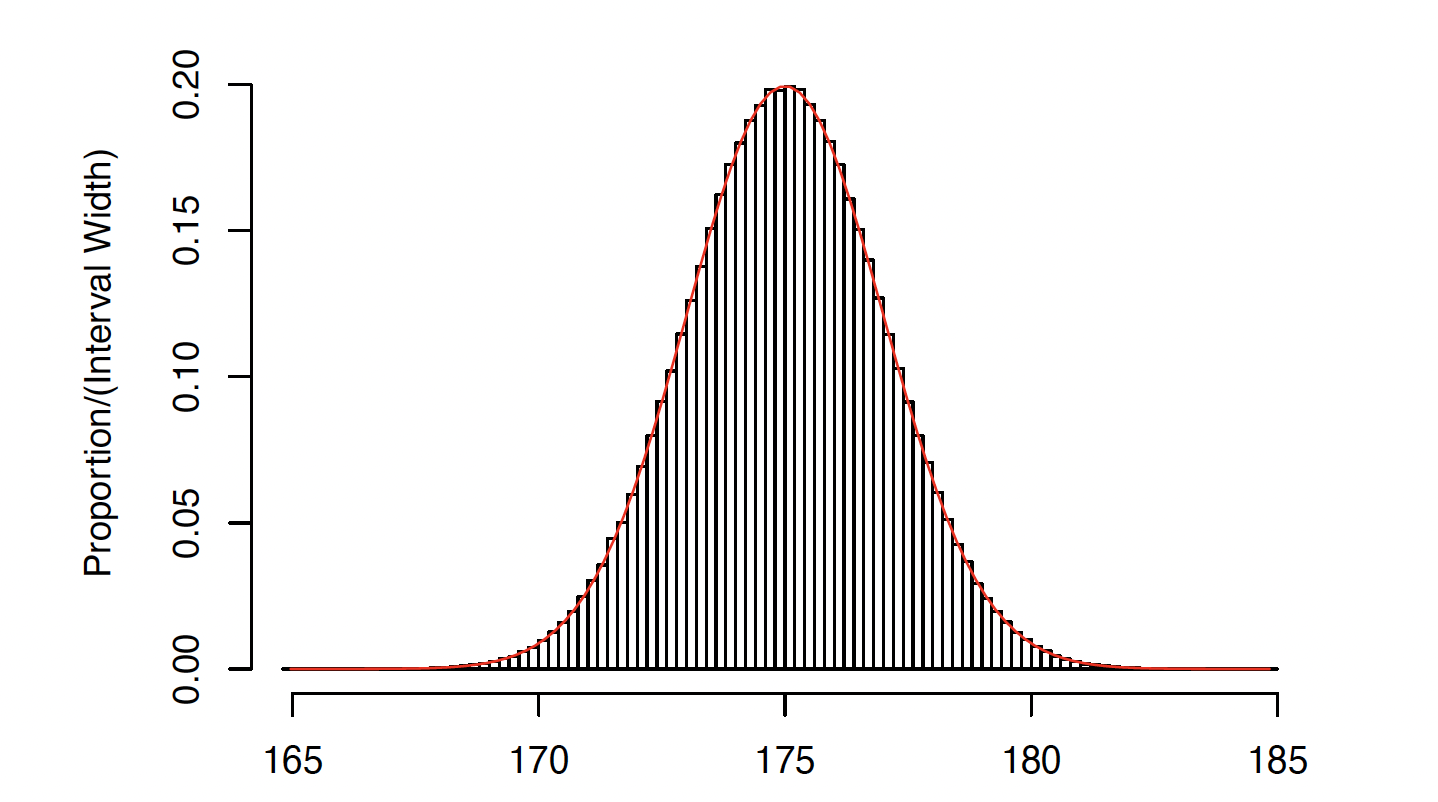
\includegraphics[width=10cm]{histo5.png}
\end{frame}

\begin{frame}
	\frametitle{Probability Density Function}
	\begin{itemize}
		\item[\color{blue}$\blacktriangleright$] As the number of observations and intervals both approach infinity, histograms of continuous data will approach a smooth curve (red line).
		\item[\color{blue}$\blacktriangleright$] The function that describes this curve is called the probability density function (PDF) and is denoted by $f(x)$.
		\item[\color{blue}$\blacktriangleright$] Can be thought of as the continuous analogue of the discrete probability distribution.
	\end{itemize}

\end{frame}
\begin{frame}
	\frametitle{Examples of PDFs}
	\centering
	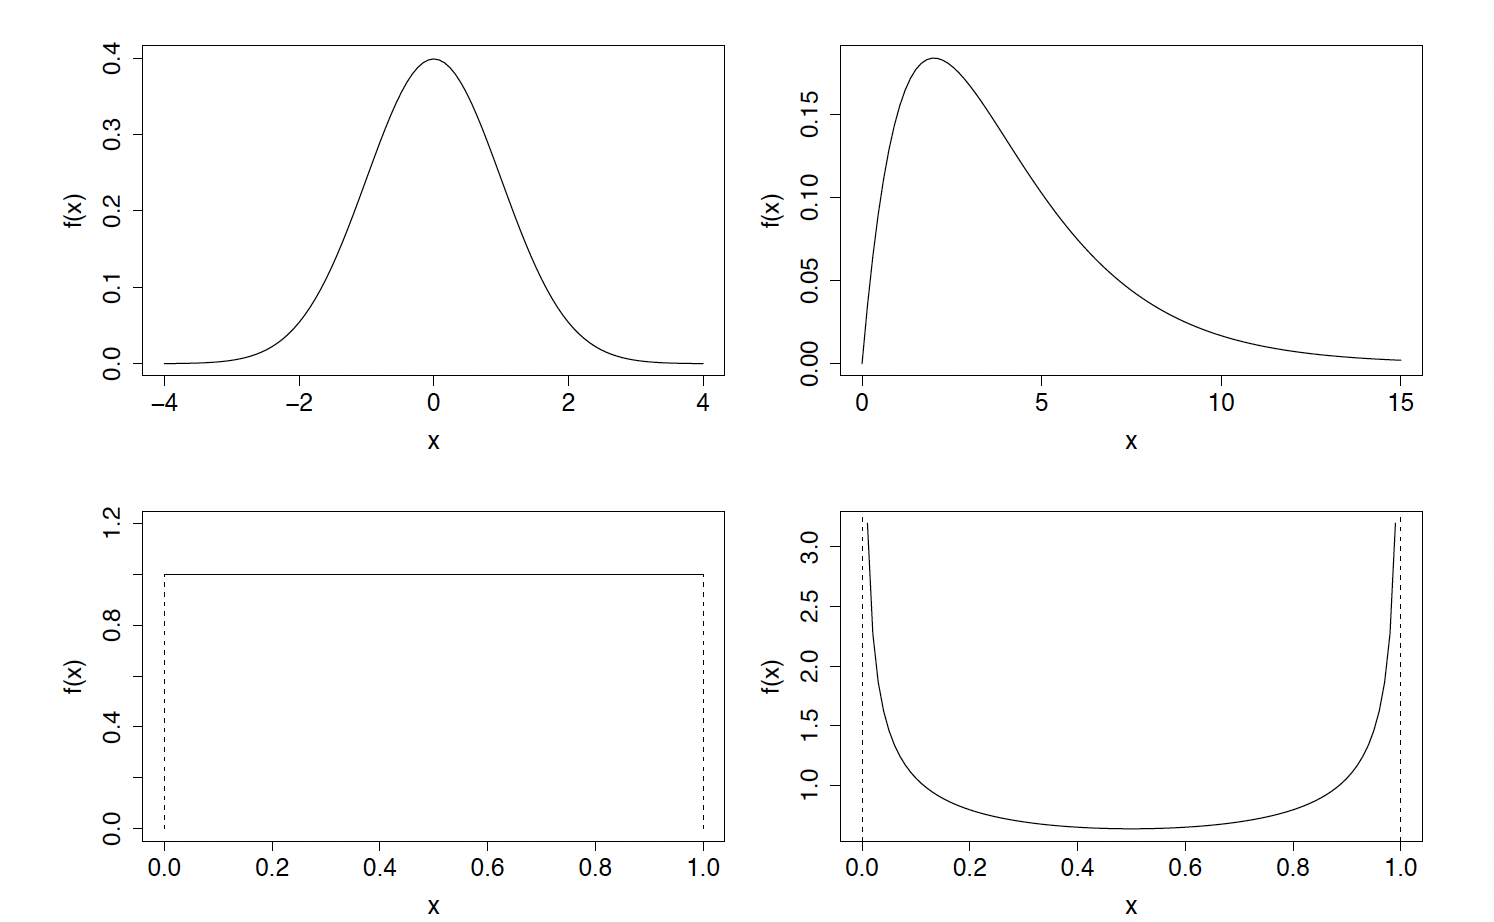
\includegraphics[width=11cm]{pdf.png}
\end{frame}

\begin{frame}
	\frametitle{Important Properties}
	\begin{itemize}
		\item[\color{blue}$\blacktriangleright$] The PDF, $f(x)$, of a continuous random variable $X$ must satisfy:
		\begin{enumerate}[label=\textcolor{blue}{\arabic*.}]
			\item $f(x)\ge0$ for all $x$ (non-negative)
			\item $\int_{-\infty}^{\infty}f(x)dx=1$ ((total area under curve equals 1).
		\end{enumerate}
	\end{itemize}
	\centering
	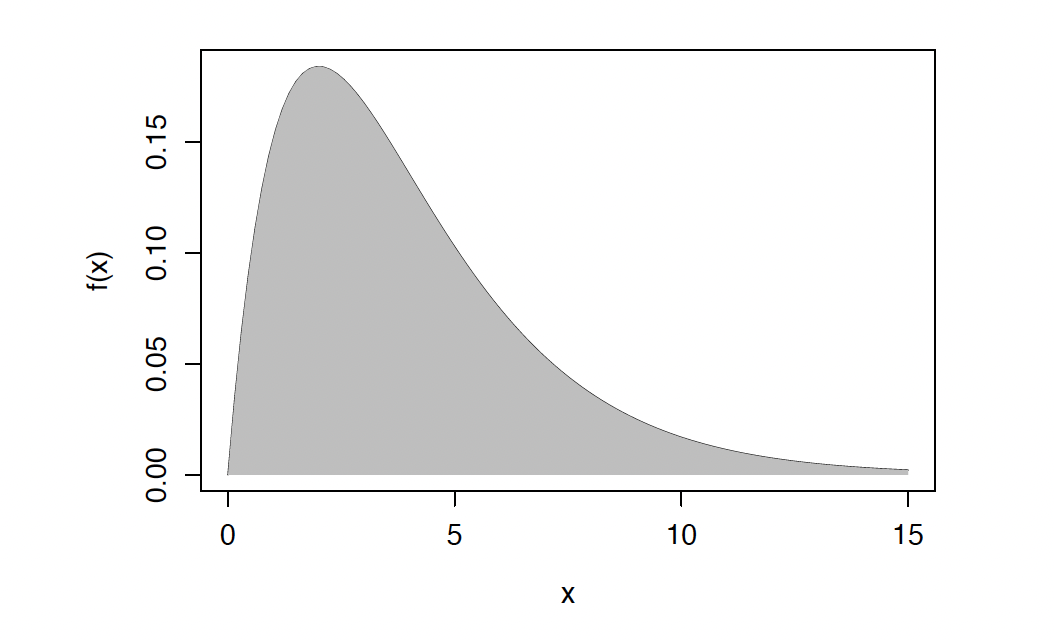
\includegraphics[width=8cm]{pdf2.png}
\end{frame}

\begin{frame}
	\frametitle{Why is the PDF Important?}
	\begin{itemize}
		\item[\color{blue}$\blacktriangleright$] Just like with the discrete probability distribution, probability density functions represent populations.
		\item[\color{blue}$\blacktriangleright$] Once we know the probability density function of a continuous random variable, we know everything about that variable.
		\item[\color{blue}$\blacktriangleright$] We can use it to calculate probabilities and also population parameters like the mean (expected value) and variance.
	\end{itemize}
	
\end{frame}
\begin{frame}
	\frametitle{Calculating Probabilities}
	\begin{itemize}
		\item[\color{blue}$\blacktriangleright$] The probability that $X$ lies between $a$ and $b$ is equal to area under the PDF between the points $a$ and $b$.
		\item[\color{blue}$\blacktriangleright$] It is calculated by $P(a<X<b)=\int_{a}^{b}f(x)dx$
	\end{itemize}
\centering
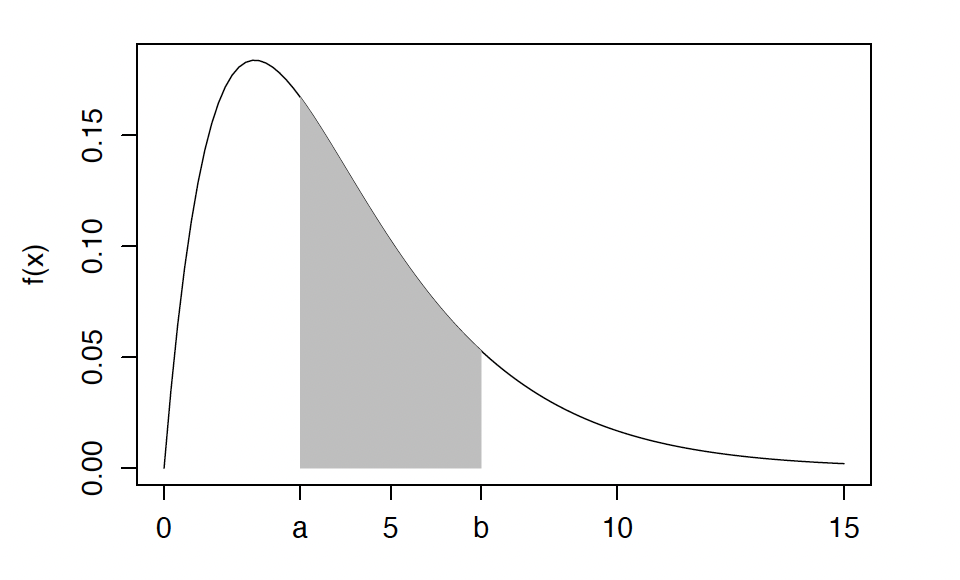
\includegraphics[width=8cm]{pdf3.png}
\end{frame}
\begin{frame}
	\frametitle{Calculating Probabilities}
	\begin{itemize}
		\item[\color{blue}$\blacktriangleright$] Recall that the probability $X$ will equal any specific value is always zero, i.e., $P(X=x)=0$ for all $x$.
		\item[\color{blue}$\blacktriangleright$] We can see that as $a\rightarrow b$, then the area $\rightarrow0$.
	\end{itemize}
	\centering
	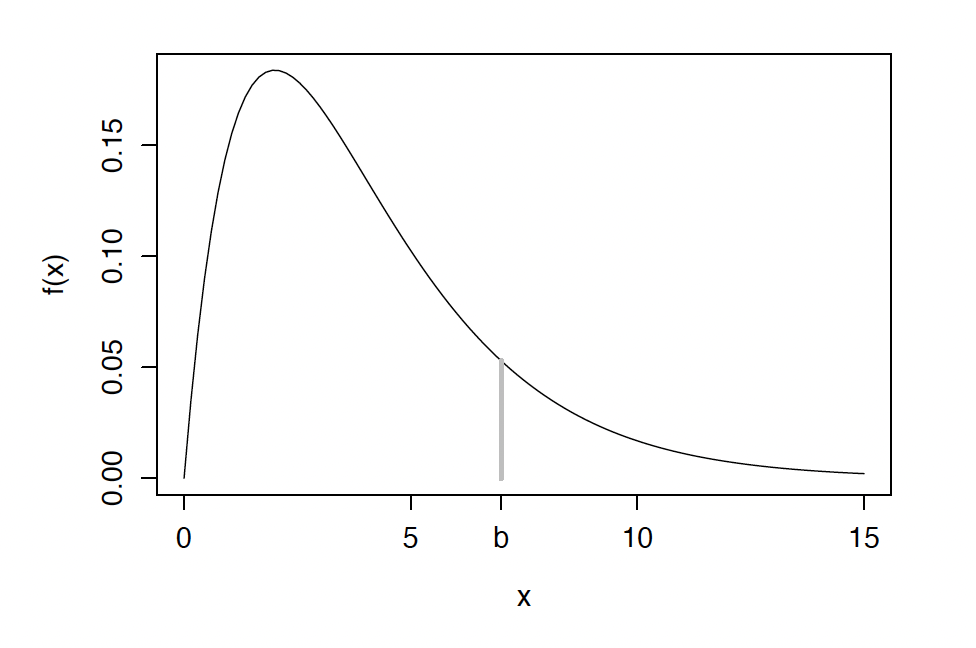
\includegraphics[width=8cm]{pdf4.png}
\end{frame}
\begin{frame}
	\frametitle{Calculating Probabilities}
\[
f(x) = \begin{cases}
	-x + 1, & 0 \leq x < 1 \\
	x - 1, & 1 \leq x \leq 2
\end{cases}
\]
	\centering
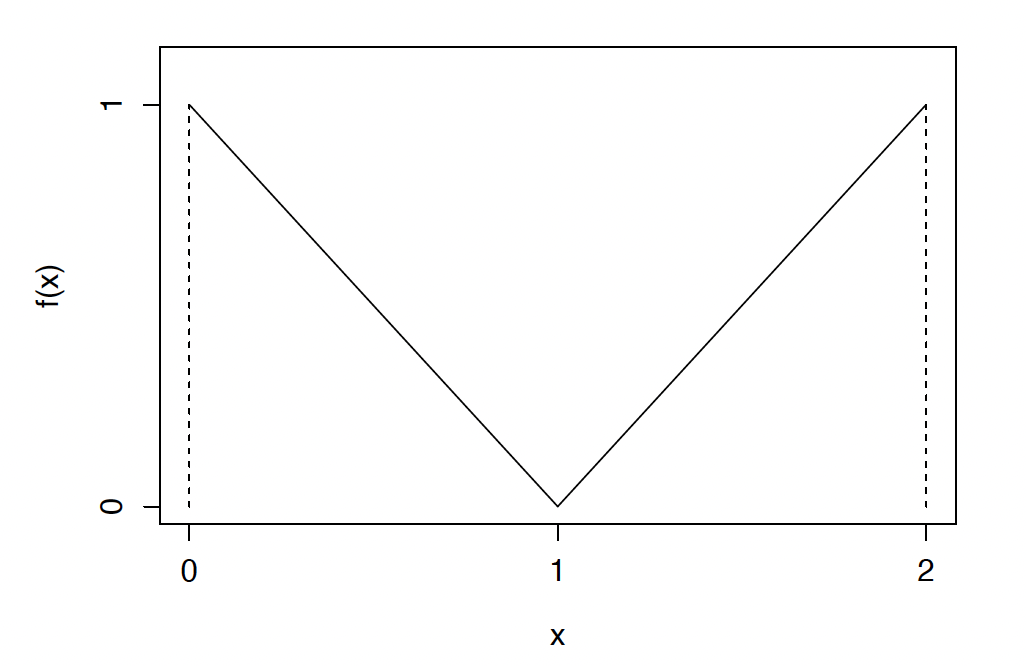
\includegraphics[width=8cm]{pdf5.png}
\end{frame}
\begin{frame}
	\frametitle{Is $f(x)$ a Valid PDF?}
	\begin{itemize}
	\item[\color{blue}$\blacktriangleright$] From the graph, $f(x)\ge0$ for all $0\le x\le2$.
	\item[\color{blue}$\blacktriangleright$] The total area under the curve is equal to:
	$$\frac{1}{2}\times1\times1+\frac{1}{2}\times1\times1=1$$
\end{itemize}
	\centering
	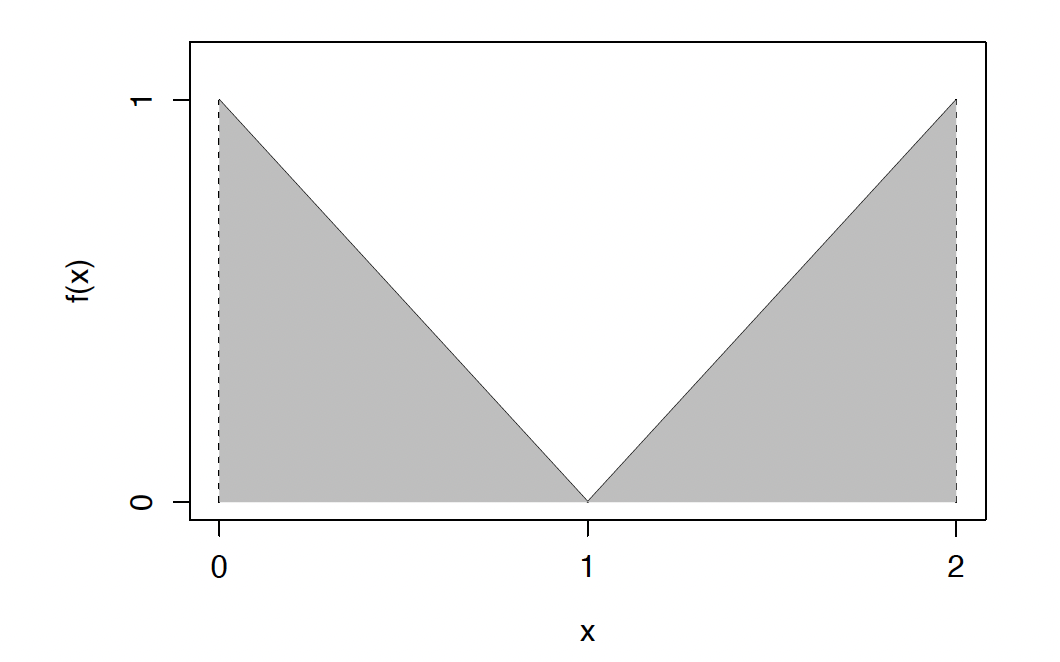
\includegraphics[width=8cm]{pdf6.png}
\end{frame}
\begin{frame}
	\frametitle{Find $P(X<0.5)$}
		\centering
	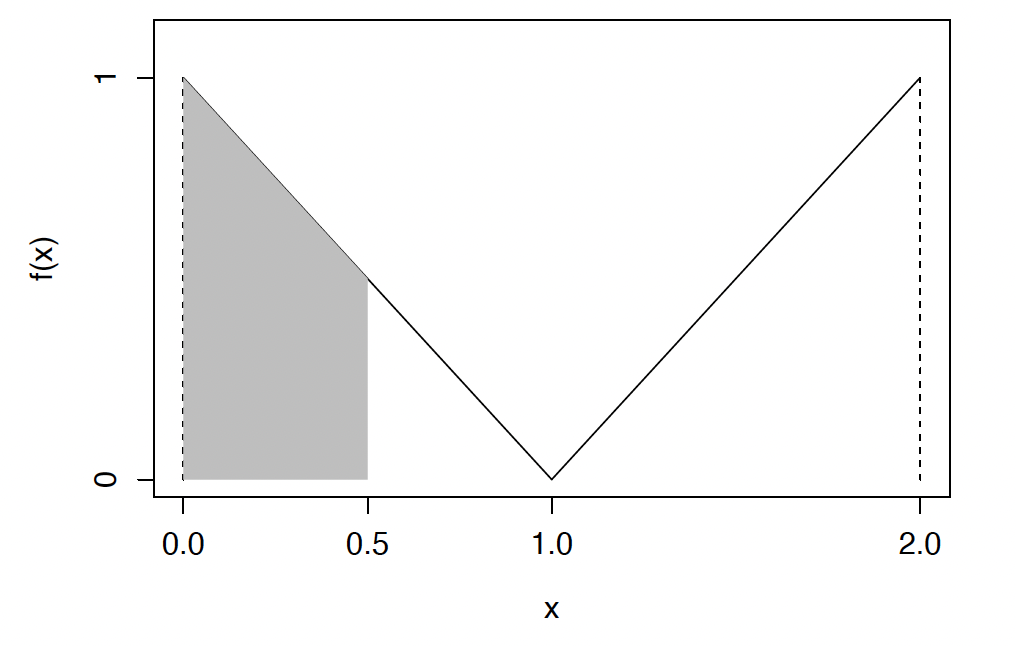
\includegraphics[width=8cm]{pdf7.png}
		\begin{align*}
		P(X<0.5)&=P(X<1)-P(0.5<X<1)\\
		&=\frac{1}{2}\times1\times1-\frac{1}{2}\times0.5\times0.5=\frac{3}{8}
		\end{align*}
\end{frame}
\begin{frame}
	\frametitle{Find $P(0.6<X<1.7)$}
	\centering
	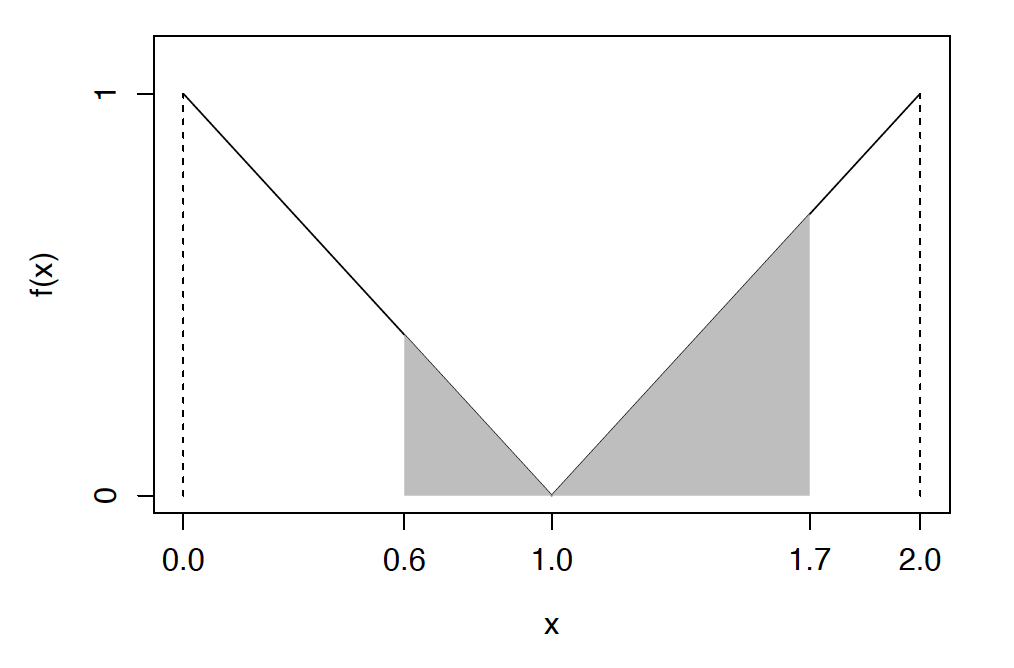
\includegraphics[width=8cm]{pdf8.png}
	\begin{align*}
		P(0.6<X<1.7)&=P(0.6<X<1)+P(1<X<1.7)\\
		&=\frac{1}{2}\times0.4\times0.4+\frac{1}{2}\times0.7\times0.7=\frac{13}{40}
	\end{align*}
\end{frame}
\begin{frame}
	\frametitle{Expected Value}
	
	\begin{itemize}
		\item[\color{blue}$\blacktriangleright$] Let $X$ be a continuous random variable with PDF $f(x)$. The \textbf{expected value} (or \textbf{population mean}) of $X$ is defined to be:
		
		\[\mu = E(X) = \int_{-\infty}^{\infty} x f(x) dx\]
		
		\item[\color{blue}$\blacktriangleright$] The \textbf{expected value} of $g(X)$, where $g(X)$ is some function of $X$, is defined to be:
		
		\[\mu = E(g(X)) = \int_{-\infty}^{\infty} g(x) f(x) dx\]
	\end{itemize}
	
\end{frame}

\begin{frame}
	\frametitle{Variance}
	
	\begin{itemize}
		\item[\color{blue}$\blacktriangleright$] Let $X$ be a continuous random variable with PDF $f(x)$ and $\mu = E(X)$. The \textbf{(population) variance} of $X$ is defined to be:
		
		\[\sigma^2 = V(X) = E((X-\mu)^2) = \int_{-\infty}^{\infty} (x-\mu)^2 f(x)dx\]
		
		\item[\color{blue}$\blacktriangleright$] A shortcut formula for the variance is given below:
		
		\[V(X) = E(X^2) - (E(X))^2 = \left(\int_{-\infty}^{\infty} x^2 f(x)dx\right) - \mu^2\]
	\end{itemize}
	
\end{frame}

\begin{frame}
	\frametitle{Special Continuous Distributions}
	
	\begin{itemize}
		\item[\color{blue}$\blacktriangleright$] There are a number of special continuous distributions, some of which we will encounter in this course:
		\begin{itemize}
			\item[\color{blue}$\blacktriangleright$] Uniform distribution.
			\item[\color{blue}$\blacktriangleright$] Normal distribution.
			\item[\color{blue}$\blacktriangleright$] $t$-distribution.
			\item[\color{blue}$\blacktriangleright$] $F$-distribution.
			\item[\color{blue}$\blacktriangleright$] Chi-squared distribution.
			\item[\color{blue}$\blacktriangleright$] Exponential distribution.
			\item[\color{blue}$\blacktriangleright$] Cauchy distribution.
		\end{itemize}
	\end{itemize}
	
\end{frame}

\begin{frame}
	\frametitle{Uniform Distribution}
	
	\begin{itemize}
		\item[\color{blue}$\blacktriangleright$] A continuous random variable $X$ is said to have a \textbf{uniform distribution} between $a$ and $b$ if its PDF is given by the following function:
		
		\[f(x) = \frac{1}{b-a}, \quad a \leq x \leq b\]
		
		\item[\color{blue}$\blacktriangleright$] We use the notation $X \sim U(a,b)$.
		
		\item[\color{blue}$\blacktriangleright$] There are two \textit{parameters} that define a uniform distribution, namely, $a$ and $b$.
	\end{itemize}
	
\end{frame}

\begin{frame}
	\frametitle{Probability Density Function of Uniform Distribution}
	\centering
	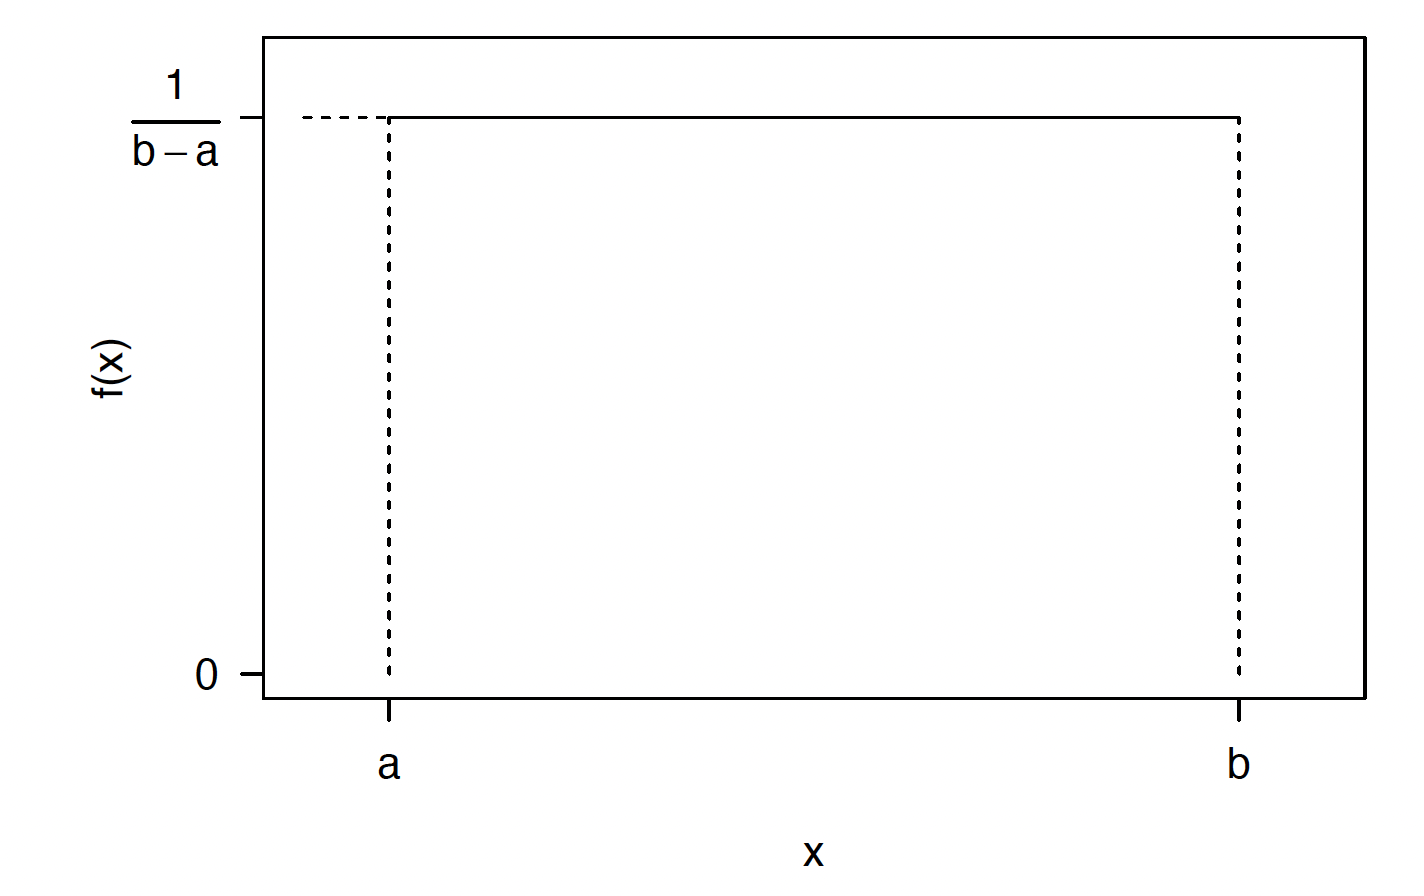
\includegraphics[width=12cm]{pdf9.png}
\end{frame}
\begin{frame}
	\frametitle{Expected Value and Variance}
	
	\begin{itemize}
		\item[\color{blue}$\blacktriangleright$] Let $X \sim U(a,b)$.
		\item[\color{blue}$\blacktriangleright$] The \textbf{expected value} of $X$ is given by:
		\[E(X) = \frac{a + b}{2}\]
		\item[\color{blue}$\blacktriangleright$] The \textbf{variance} of $X$ is given by:
		\[V(X) = \frac{(b - a)^2}{12}\]
	\end{itemize}
	
\end{frame}
\begin{frame}
	\frametitle{Expected Value}
	
	\begin{align*}
		E(X) &= \int_{-\infty}^{\infty} x f(x) dx \\
		&= \int_a^b x \times \frac{1}{b-a} dx \\
		&= \frac{1}{b-a} \left[\frac{x^2}{2}\right]|_a^b \\
		&= \frac{b^2 - a^2}{2(b-a)} \\
		&= \frac{(b+a)(b-a)}{2(b-a)} \\
		&= \frac{a+b}{2}
	\end{align*}
	
\end{frame}
\end{document}